\documentclass{article}

\usepackage{amsmath, amssymb, amsthm}
\usepackage{algorithm2e}
\usepackage{enumitem}
\usepackage{tcolorbox}
\usepackage{tikz}

\newtheorem*{fact7.5}{Fact 7.5}

\title{Exercise of Chapter 7}
\author{Xiaoyu Chen}
\date{}

\begin{document}
\maketitle

\section{Exercise 7.6}
Provide a formal statement of Fact 1.5 using the notion of witness-checking predicates.
\subsection{Solution}
First we provide a formal version for Fact 1.5.
\begin{fact7.5}[Formal Statement]
  Suppose we have a witness-checking predicate $\chi: \Sigma^*\times\Sigma^*\to \{0, 1\}$,
  from which we could define two problem $\varphi$ and $f$ such that $\forall x\in \Sigma^*$,
  \begin{align*}
    \varphi(x) &\Leftrightarrow \exists\omega\in\Sigma^*.\chi(x,\omega)\land|\omega|\leq P(|x|) \\
    f(x) &= |\omega\in\Sigma^*: \chi(x,\omega)\land |w|\leq P(|x|)|
  \end{align*}
  Then $f$ does not admit a $FPRAS$ unless $PR = NP$.
\end{fact7.5}
Though the problem itself does not require a proof of this fact,
I give one here for a better understanding.
\begin{proof}
  If $f$ has a $FPRAS$,
  then we have a function $S$ such that,
  \[\Pr[e^{-\varepsilon}f(x)\leq S(x)\leq e^\varepsilon f(x)] \geq \frac{3}{4}\]
  which could be calculated in polynomial time.
  So we could define a witness-checking predicate $\chi'$ for $\varphi$ as
  \[X'(x, \omega) := [S(x) > 0]\]
  Then we have:
  \begin{enumerate}[itemsep=0mm]
  \item If $\varphi(x)$, then $f(x) > 0$, then $e^{-\varepsilon}>0$ and $e^\varepsilon > 0$.
    Thus, $\Pr[S(x) > 0] \geq \Pr[e^{-\varepsilon}f(x)\leq S(x)\leq e^{\varepsilon}] \geq \frac{3}{4}$.
  \item If $\lnot\varphi(x)$, then $f(x) = 0$, then $e^{-\varepsilon} = e^\varepsilon = 0$.
    Thus, $\Pr[S(x) = 0] \geq \frac{3}{4}$ and hence $\Pr[S(x) > 0]\leq \frac{1}{4}$.
  \end{enumerate}
  So, $\varphi$ is in BPP.

  Then, to go further, we want $\varphi$ to be some practical $NPC$ problem, i.e. SAT problem.
  (I get this idea from a online material).
  Suppose we have a SAT problem $\phi$ which has $k$ variables $x_1, x_2, \cdots, x_k$.
  To make things more easy, we could construct another witness-checking predicate $\chi''$ from $\chi'$ by calling $\chi'$ polynomial times, such that
  \begin{enumerate}[itemsep=0mm]
  \item If $\varphi(\phi)$, then $\Pr[\chi''(\phi, \omega)] \geq 1 - 2^{-m}$
  \item If $\lnot\varphi(\phi)$, then $\Pr[\chi''(\phi, \omega)] \leq 2^{-m}$.
  \end{enumerate}
  We try to construct a witness-checking predicate $\chi^*$ for SAT problem.
  \begin{algorithm}[ht]
    witness-checking predicate $X^*(\phi, \omega)$ \Begin{
      \If{$\lnot\chi''(\phi, \omega)$}{
        \Return{false}
      }
      \For{$i$ in $[1, n]$} {
        $x_i \gets 0$ \\
        Get a new problem $\phi_1$ by fix variables from $x_1$ to $x_i$ \\
        \If{$\lnot\chi''(\phi_1, \omega_1)$} {
          \tcc{Here $\omega_1$ is some random solution for $\phi_1$}
          $x_i \gets 1$ \tcp{also modify $x_i$ in $\phi_1$}
        }
      }
      $\omega_1\gets \{x_1, x_2, \cdots, x_n\}$ \\
      \Return{$\chi(\phi, \omega_1)$}
    }
  \end{algorithm}
  
  When $\lnot\varphi(\phi)$, if $\lnot\chi''(\phi, \omega)$, $\chi^*(\phi,\omega)$ returns \textit{false}.
  If $\chi''(\phi,\omega)$, then $\chi^*$ will construct a solution $\omega_1$ by using $\chi''$ polynomial times.
  And if $\lnot\chi(\phi,\omega_1)$, then $\chi^*$ will return \textit{false}.
  So, these ensures that $\lnot\varphi(\phi) \Rightarrow \lnot\chi^*(\phi, \omega)$ for all $\omega$.

  When $\varphi(\phi)$, consider the probablity for $\chi^*(\phi, \omega)$.
  We only need to analysis the worst case for this, i.e. when there is only one $\omega$ such that $\chi(\phi,\omega)$.
  To achieve $\chi^*(\phi,\omega)$, we need to avoid wrong choice made by $\chi''$.
  Note that we have $k+1$ choices made by $\chi''$ and each of them have probability at less than $2^{-m}$ to be wrong.
  So, in this case,
    \[\Pr[\chi^*(\phi, \omega)] \geq (1-2^{-m})^{k+1} \geq \frac{1}{2}\]
  for some appropriate $m$.

  So, its clear that $\chi^*$ reaches the requirement of $RP$ and we have $\varphi$ is in $RP$,
  which implies that $NP\subseteq RP$.
  Together with $RP\subseteq NP$, we have $RP = NP$.
\end{proof}

\section{Exercise 7.10}
Complete the proof of Theorem 7.9. To keep technical complexity to a minimum, assume the graph G is triangle-free, i.e., contains no cycles of length 3.
\subsection{Solution}
Suppose there are two states $x, y\in\Omega$, the distance $d(x, y)$ between them is defined as the hamming distance between them.
Then, to use the path-coupling method, we need to design the coupling.
The coupling is defined between the pairs $(X_0, Y_0)$, where $d(X_0, Y_0) = 1$.
Since $d(X_0, Y_0) = 1$, we could assume that there exists a vertex $v$ where $X_0(v) = 0$ and $Y_0(v) = 1$ without loss of generality.
\begin{algorithm}[ht!]
  \tcc{Update the status of two vertices}
  Update($X, u, w, a, b$)\Begin{
    $X_1\gets X$, where $X_1(u) = a$ and $X_1(v) = b$ \\
    \If{$X_1$ is a independent set}{
      \Return{$X_1$}
    }
    \Return{$X$}
  }
  \tcc{define the coupling for $d(X_0, Y_0) = 1$}
  Coupling$(X_0, Y_0)$\Begin{ 
    Choose an edge $\{u, w\}\in E$, u.a.r. \\
    \tcc{general cases for selecting $(a, b)$}
    Select $(a, b)$ from $\{(0, 0), (0, 1), (1, 0)\}$, u.a.r. \\
    \tcc{If $v\in \{u, w\}$, then we only select $(a, b)$ from the feasible combinations}
    \If{$u=v\lor w=v$}{
      \tcc{assume $u=v$, without loss of generality}
      \If{$X_0(\mathbb{N}(w)\setminus\{u\}) = 1$} {
        Select $(a, b)$ from $\{(0, 0), (1, 0)\}$, u.a.r. \\
      }
    }
    Update$(X_1, u, w, a, b)$, Update$(Y_1, u, w, a, b)$ \\
    \Return{$(X_1, Y_1)$}
  }
\end{algorithm}


After that, we are going to analysis the value of $\mathbb{E}[d(X_1, Y_1)]$.
Denote the neighbor of $v$ by $\mathbb{N}(v)$, and $\mathbb{N}[v] := \{v\}\cup \mathbb{N}(v)$. Then, any edge $\{u, w\}$ of $G$ must belongs to one of the following three classes.
\begin{enumerate}[itemsep=0mm]
\item $u\not\in\mathbb{N}[v]\land w\not\in\mathbb{N}[v]$, i.e., $v$ is not the neighbor of edge $\{u, w\}$.
\item $u\in \mathbb{N}(v)\land w\not\in \mathbb{N}[v]$, i.e., $v$ is a neighbor of edge $\{u, w\}$.
\item $u = v\land w\in\mathbb{N}(v)$, i.e., $v$ is an end point of edge $\{u, w\}$.
\end{enumerate}
Since $G$ is triangle-free, we do not need to consider the case $u\in\mathbb{N}(v)\land w\in\mathbb{N}(v)$.
\paragraph{For the first case:}
Note that $X_1$ and $Y_1$ will satisfies the requirement for a independent set simutaneously, because the status of all the neighbors of edge $\{u, w\}$ are the same in $X_0$ and $Y_0$. So in this case
\[d(X_1, Y_1) = d(X_0, Y_0)\]
\paragraph{For the second case:}
Recall that $X_0(v) = 0$ and $Y_0(v) = 1$.
Intuitively, we have the following circumstance
\begin{center}
  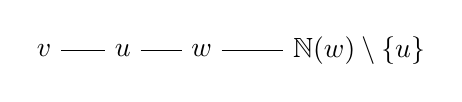
\begin{tikzpicture}
    \node (v) at (0, 0) {$v$};
    \node (u) at (1, 0) {$u$};
    \node (w) at (2, 0) {$w$};
    \node (r) at (4, 0) {$\mathbb{N}(w)\setminus\{u\}$};
    \draw (v) to (u);
    \draw (u) to (w);
    \draw (w) to (r);
  \end{tikzpicture}
\end{center}
Since $X_0(\mathbb{N}(w)\setminus\{u\}) = Y_0(\mathbb{N}(w)\setminus\{u\})$, we only need to consider whether there is any vertex in $\mathbb{N}(w)\setminus\{u\}$ in the independent set. Let $\delta = d(X_1, Y_1) - d(X_0, Y_0)$.
\begin{center}
  \begin{tabular}{|c|c|c|}
    \hline
    $X_0(\mathbb{N}(w)\setminus\{u\})$ & possible cases to make $\delta = -1$ & possible cases to make $\delta = 1$ \\
    \hline
    0 & None & $(1, 0)$ \\
    \hline
    1 & None & $(1, 0)$ \\
    \hline
  \end{tabular}
\end{center}
Lets denote the number of edges belong to the second case by $n_2$, then
\begin{align*}
  \mathbb{E}(\delta) &= \frac{n_2}{m} \times \frac{1}{3} \\
  &= \frac{n_2}{3m}
\end{align*}

\paragraph{For the third case:}
Since in this case, we only select $(a, b)$ from feasible combinations, the probability of $d(X_1, Y_1) = 0$ is 1. So if we denote the number of edges belong to the second case by $n_3$, then
\[\mathbb{E}(\delta) = \frac{-n_3}{m}\]

Put all the cases together, we have
\begin{align*}
  \mathbb{E}(\delta) &= \frac{1}{m}(\frac{n_2}{3} - n_3) \\
  &\leq \frac{1}{m}(\frac{3n_3}{3} - n_3), \hspace{0.5cm} \mbox{Since $n_2\leq 3n_3$} \\
  &= 0
\end{align*}

\begin{tcolorbox}[title={Note}]
Note that although we complete the proof on the book, it does not mean that we have proved the MC is rapidly mixing. The complete proof bases on a carefully designed distance measure function.
\end{tcolorbox}

\section{Exercise 7.12}
Using the same reduction, but improved estimates, show that Proposition 7.11 holds for some $\Delta$ less than 1100. (I think $\Delta = 964$ is achievable)
\subsection{Solution}
First, we could note that we have a loose upper bound for $|J'|$.
Actually, we could fix this upper bound, and we have
\[(2^r - 1)^k \leq |J'| \leq \binom{n}{k}(2^r - 1)^k\]
Recall that we have Stirling Formula for $n!$:
\[\sqrt{2\pi n}\left(\frac{n}{e}\right)^n \leq n! \leq 2\sqrt{2\pi n}\left(\frac{n}{e}\right)^n\]
So
\begin{align*}
  \binom{n}{k} &= \frac{n!}{k!(n-k)!} \\
  &\leq \frac{2\sqrt{2\pi n}\left(\frac{n}{e}\right)^n}{\sqrt{2\pi k}\left(\frac{k}{e}\right)^k \sqrt{2\pi(n-k)}\left(\frac{n-k}{e}\right)^{n-k}} \\
  &\leq \frac{2\sqrt{n}n^n}{\sqrt{k}\sqrt{2\pi(n-k)}k^k (n-k)^{n-k}}\\
  &\leq \frac{2\sqrt{4k}(4k)^{4k}}{\sqrt{k}\sqrt{2\pi(4k-k)}k^k (4k-k)^{4k-k}}, \hspace{0.5cm} \mbox{since $k \geq \frac{n}{4}$}\\
  &= \frac{4\times 4^{4k}k^{4k}}{\sqrt{6\pi k}\times k^k 3^{3k} k^{3k}} \\
  &= \frac{4\times 4^{4k}}{\sqrt{6\pi k}\times 3^{3k} } \\
  &\leq \frac{4^{4k}}{3^{3k}}, \hspace{0.5cm} \mbox{since $4\leq \sqrt{6\pi k}$}
\end{align*}
Then we have a more tight bound for $|J'|$
\begin{align*}
  (2^r - 1)^k \leq |J'| \leq \binom{n}{k}(2^r - 1)^k 
\end{align*}
or, taking the natural logarithm,
\begin{align*}
  %(2^r - 1)^k \leq |J'| \leq \frac{4^{4k}}{3^{3k}}(2^r - 1)^k
  k\ln(2^r - 1) \leq \ln|J'| \leq 4k\ln4 - 3k\ln3 + k\ln(2^r - 1)
\end{align*}
Consider the following estimate for $k$
\[\hat{k} = \frac{\ln|J'|}{4\ln4 - 3\ln3 + \ln(2^r - 1)}\]
then
\begin{align*}
  k(\frac{\ln(2^r - 1)}{4\ln4-3\ln3+\ln(2^r -1)}) \leq \hat{k} \leq k \\
  k(1-\frac{4\ln4-3\ln3}{4\ln4-3\ln3+\ln(2^r -1)}) \leq \hat{k} \leq k \\
\end{align*}
Note that when $r = 241$,
\[\frac{4\ln4 - 3\ln3}{4\ln4 - 3\ln3 + \ln(2^r - 1)} \leq \frac{1}{74}\]
So, we have $\Delta = 4r = 964$.
\end{document}

%%% Local Variables:
%%% mode: latex
%%% TeX-master: t
%%% End:
